\documentclass[journal]{IEEEtran}

\usepackage{cite,color,graphicx}

% *** GRAPHICS RELATED PACKAGES ***
%
\ifCLASSINFOpdf
  % \usepackage[pdftex]{graphicx}
  % declare the path(s) where your graphic files are
  % \graphicspath{{../pdf/}{../jpeg/}}
  % and their extensions so you won't have to specify these with
  % every instance of \includegraphics
  % \DeclareGraphicsExtensions{.pdf,.jpeg,.png}
\else
  % or other class option (dvipsone, dvipdf, if not using dvips). graphicx
  % will default to the driver specified in the system graphics.cfg if no
  % driver is specified.
  % \usepackage[dvips]{graphicx}
  % declare the path(s) where your graphic files are
  % \graphicspath{{../eps/}}
  % and their extensions so you won't have to specify these with
  % every instance of \includegraphics
  % \DeclareGraphicsExtensions{.eps}
\fi

\usepackage{graphicx}
\usepackage[cmex10]{amsmath}
\usepackage{algorithmic}
\usepackage{array}
\usepackage{mdwmath}
\usepackage{mdwtab}
\usepackage{eqparbox}
%\usepackage[tight,footnotesize]{subfigure}
%\usepackage[caption=false]{caption}
%\usepackage[font=footnotesize]{subfig}
%\usepackage[caption=false,font=footnotesize]{subfig}
\usepackage{fixltx2e}
\usepackage{stfloats}
\usepackage{url}

% *** Do not adjust lengths that control margins, column widths, etc. ***
% *** Do not use packages that alter fonts (such as pslatex).         ***
% There should be no need to do such things with IEEEtran.cls V1.6 and later.
% (Unless specifically asked to do so by the journal or conference you plan
% to submit to, of course. )

% correct bad hyphenation here
\hyphenation{op-tical net-works semi-conduc-tor}

\begin{document}
%
% paper title
% can use linebreaks \\ within to get better formatting as desired
\title{TODO: A Survey of StarCraft AI Techniques}
%
%
% author names and IEEE memberships
% note positions of commas and nonbreaking spaces ( ~ ) LaTeX will not break
% a structure at a ~ so this keeps an author's name from being broken across
% two lines.
% use \thanks{} to gain access to the first footnote area
% a separate \thanks must be used for each paragraph as LaTeX2e's \thanks
% was not built to handle multiple paragraphs
%

\author{FirstName~LastName,~\IEEEmembership{Member,~IEEE,}
        Jim~Raynor,~\IEEEmembership{Fellow,~RR,}
        and~Sarah~Kerrigan,~\IEEEmembership{Life~Fellow,~ZS}% <-this % stops a space
\thanks{FirstName~LastName is with the Department of Names
GA, 30332 USA e-mail: (see http://www.michaelshell.org/contact.html).}% <-this % stops a space
\thanks{J. Raynor and S. Kerrigane are with the Romeo\&Juliet Inc.}% <-this % stops a space
\thanks{Manuscript received April 19, 2499; revised January 11, 2500.}}

% note the % following the last \IEEEmembership and also \thanks - 
% these prevent an unwanted space from occurring between the last author name
% and the end of the author line. i.e., if you had this:
% 
% \author{....lastname \thanks{...} \thanks{...} }
%                     ^------------^------------^----Do not want these spaces!
%
% a space would be appended to the last name and could cause every name on that
% line to be shifted left slightly. This is one of those "LaTeX things". For
% instance, "\textbf{A} \textbf{B}" will typeset as "A B" not "AB". To get
% "AB" then you have to do: "\textbf{A}\textbf{B}"
% \thanks is no different in this regard, so shield the last } of each \thanks
% that ends a line with a % and do not let a space in before the next \thanks.
% Spaces after \IEEEmembership other than the last one are OK (and needed) as
% you are supposed to have spaces between the names. For what it is worth,
% this is a minor point as most people would not even notice if the said evil
% space somehow managed to creep in.

% The paper headers
\markboth{TCIAIG ~Vol.~X, No.~Y, Month~Year}%
{Shell \MakeLowercase{\textit{et al.}}: TODO: Title here}

\maketitle

\begin{abstract}
TODO: Idea of the paper is: ``one-stop guide on what is the
state of the art in Starcraft AI''. It should help people participating in the competition focus
their efforts, and also should help people implementing AI for RTS games in
general (e.g. industry).  In Gabriel's words ``RTS AI problems, Solutions, State-of-the-art, conclude on what's "solved" (since Buro 2004) and what's not.'' 

For example, if someone wants to implement a bot, and wonders "how should I do scouting", our paper should provide a summary of the existing techniques, and pointers to know more. 
\end{abstract}

\begin{IEEEkeywords}
review, RTS, games, StarCraft, machine learning, planning, TODO ...

\end{IEEEkeywords}

% For peer review papers, you can put extra information on the cover
% page as needed:
% \ifCLASSOPTIONpeerreview
% \begin{center} \bfseries EDICS Category: 3-BBND \end{center}
% \fi
%
% For peerreview papers, this IEEEtran command inserts a page break and
% creates the second title. It will be ignored for other modes.
\IEEEpeerreviewmaketitle

\section{Introduction}\label{sec:intro}
\IEEEPARstart{S}{ince} Michael Buro's call for research in RTS games \cite{Buro03rts}, many researchers have answered the call. Specially, AI competitions like the Starcraft one have caused many AI techniques to be
applied to RTS AI. We will list and classify these approaches, explain their 
power and their downsides and conclude on what is left to achieve human-level 
RTS AI.

{\color{blue}
Motivate the paper, and provide an outline.

Some arguments to use in the motivation could be that games are a good application to motivate novel AI research (as has been happening throughout the history of AI), and that techniques and algorithms developed for RTS games, in addition to be useful and relevant to the game industry, have broader application to other areas.

Reiterate that the goal of this paper is to provide a one-stop guide on what is the
state of the art in Starcraft AI
}

\section{Real-Time Strategy Games}\label{sec:rts}

\subsection{Starcraft}\label{subsec:starcraft}

{\color{blue}
Introduce the game plus screenshot. Not too lengthy
}

\subsection{Complexity of RTS Game AI}\label{subsec:complexity}

{\color{blue}
Here discuss the complexity of RTS games in general, but focusing on Starcraft. The most important thing of this section is to demonstrate that RTS games are complex, and this is the motivation for requiring all the challenges and research presented afterwards.
}

\subsection{Challenges in RTS Game AI}\label{subsec:challenges}

{\color{blue}
Many years have passed since Buro's call for research (8!!). he identified 6 challenges:
\begin{itemize}
\item Resource management
\item Decision making under uncertainty
\item Spatial and temporal reasoning
\item Collaboration
\item Opponent modeling, Learning
\item Adversarial real-time planning
\end{itemize}

There has been a lot of work in many, but others have been untouched (e.g. Collaboration). Additionally, other challenges that are not in the list appeared, and have been worked on, like: how to exploit the existing domain knowledge (strategies, build-orders, replays, etc.), or how to design an architecture that integrates all the modules required for an agent to play an RTS games. This section should provide an updated view of challenges, and set the ground for the rest of the paper. The remainder of the paper should be structured around the challenges that we list here.

I think that a good list could be something like this (I'm open to all kind of criticism here :)):

\begin{itemize}
\item Task Decomposition (or ``Architecture'')
\item Integration of Domain Knowledge
\item Reasoning with Uncertainty (including information gathering)
\item Opponent Modeling and Adaptation
\item Group and Individual Control (``micro'')
\item Planning and Resource Allocation (``macro'')
\end{itemize}

I've now listed them as challenges, but maybe we can list them as questions. In each of the subsequent sections, we should use the bots in the competitions (BBQ, EISBot, Nova, UAlbertaBot, etc.) to illustrate the state-of-the-art. Eventually, we could refer to other work though if need be. We could also compare with what is being used in industry, and use the real AI of Starcraft as an example (Bob Fitch's talk in AIIDE provides enough material for that).
}

\section{Challenge 1: Task Decomposition}\label{sec:architecture}

{\color{blue}
Here we should say that complex RTS games require multi-scale reasoning \cite{WeberCig10}, and thus complex architectures that integrate many AI modules have been devised. Discuss how different researchers have divided up the task of playing Starcraft into a collection of subtasks and integrated them (see the end of this paper for a preliminary write-up on this)
}


\section{Challenge 2: Integration of Domain Knowledge}\label{sec:domainknowledge}

{\color{blue}
All bots attempt at integrating human domain knowledge in a way or another, be it in the form of build-orders, heuristics, strategies, or by automatically learning from human replays. This has been shown to be key to good performance in bots (for now, as Dave was saying: ``Starcraft AI is like Chess was in the 60s''). 

Talk about learning, scripting, and other techniques to incorporate such knowledge.
}

\section{Challenge 3: Reasoning with Uncertainty}\label{sec:uncertainty}

{\color{blue}
I think there are two important aspects of uncertainty in RTS games.

First is trying to model uncertainty and try to reduce it (information gathering, and representation of knowledge), this includes scouting, and maintaining good estimates of locations and number of units of the enemy, etc.

Second is actually using the uncertain information. Taking decisions like army strength estimation (like to attack or retreat).
}

\section{Challenge 4: Opponent modeling and Adaptation}\label{sec:adaptation}

{\color{blue}
What has been done in modeling the strategy of the opponent and adapt accordingly? which bots do adapt themselves to what they learn from the opponent and how?
}

{\color{red} I'm a bit worried that Challenge 3 and 4 will overlap significantly, since a large source of uncertainty is the opponent, so, part of opponent modeling has a lot to do with uncertainty. What do you think?}

\section{Challenge 5: Group and Individual Control}\label{sec:micro}

{\color{blue}
One of the big areas where we have seen a lot of research is in micro-management, where participants in the competitions have used reinforcement-learning (Overmind), potential-fields (BTHAI, Nova, and others), or many other techniques for coordinating both individual unit and group behavior.
}

\section{Challenge 6: Planning and Resource Allocation}\label{sec:planning}

{\color{blue}
This section is intended to refer to all those techniques concerning ``macro'', since resource allocation and planning is considered together in most state-of-the-art bots (do you agree?). Here we can talk about things like build-order-optimization, resource allocation to different aspects of the game (army, research, etc.)
}



\section{Empirical Comparison of RTS Bots}\label{sec:experiments}

{\color{blue}
What are the similarities and differences of the current bots in the competition? which techniques are widespread, and which are experimental? which features decide over winning? Which features would have a high impact if we work on them?
}

{\color{red} Given that we have Ben, Mike (Preuss), Dave and possibly Michael (Buro) on board, we could include results from the competitions. But, given that this is not a standard ``competition paper'', maybe you guys want to reserve that data to put together a separate paper. It's your call, since it's your data :)}
	
\section{Discussion and Outlook}\label{sec:conclusions}
	
{\color{blue}	
what is solved, what is not, what needs more work, which challenges have not even addressed. This section should go back to the list of challenges from Section \ref{subsec:challenges} and discuss them in the light of what has been said afterwards. I think this is a VERY IMPORTANT section, since it should provide our vision on the field.

For example, notice that a big challenge missing from the above sections is {\em Spatial and Temporal Reasoning}. While I think (and I'm sure you'll agree) that this should be a huge topic in RTS game AI, I haven't seen much of this beyond potential fields. Because of this (as Michael Buro mentioned), many bots fall prey of easy tricks due to lack of common sense reasoning.

It should also present an outlook of what is to come and what is needed.
}


\section*{Acknowledgments} {\color{blue} This research is partially funded by projects ... and ... }


\appendix

\section*{This is the old task-division section}

{\color{red}
I've included here the section we had for not losing it :)
}


Playing an RTS game involves dealing with all the problems described above. A few approaches, like CAT \cite{LTW}, Darmok \cite{OntanonMSR10} or ALisp \cite{Marthi05} try to deal with the problem in a monolithic manner, by using a single AI technique. This resembles approaches to solve other games, such as Chess or Go, where a single game-tree search approach is enough to play the game at human level. However, none of those systems aims at achieving near human performance. In order to achieve human-level performance, RTS AI designers use a lot of domain knowledge in order to divide the task of playing the game into a collection of sub-problems, which can be dealt-with using individual AI techniques (as discussed in the previous section). Thus, an integration architecture is required to put together all of those techniques into a single coherent system, which is the focus of this section.

\begin{figure*}[ta]
    \centering
    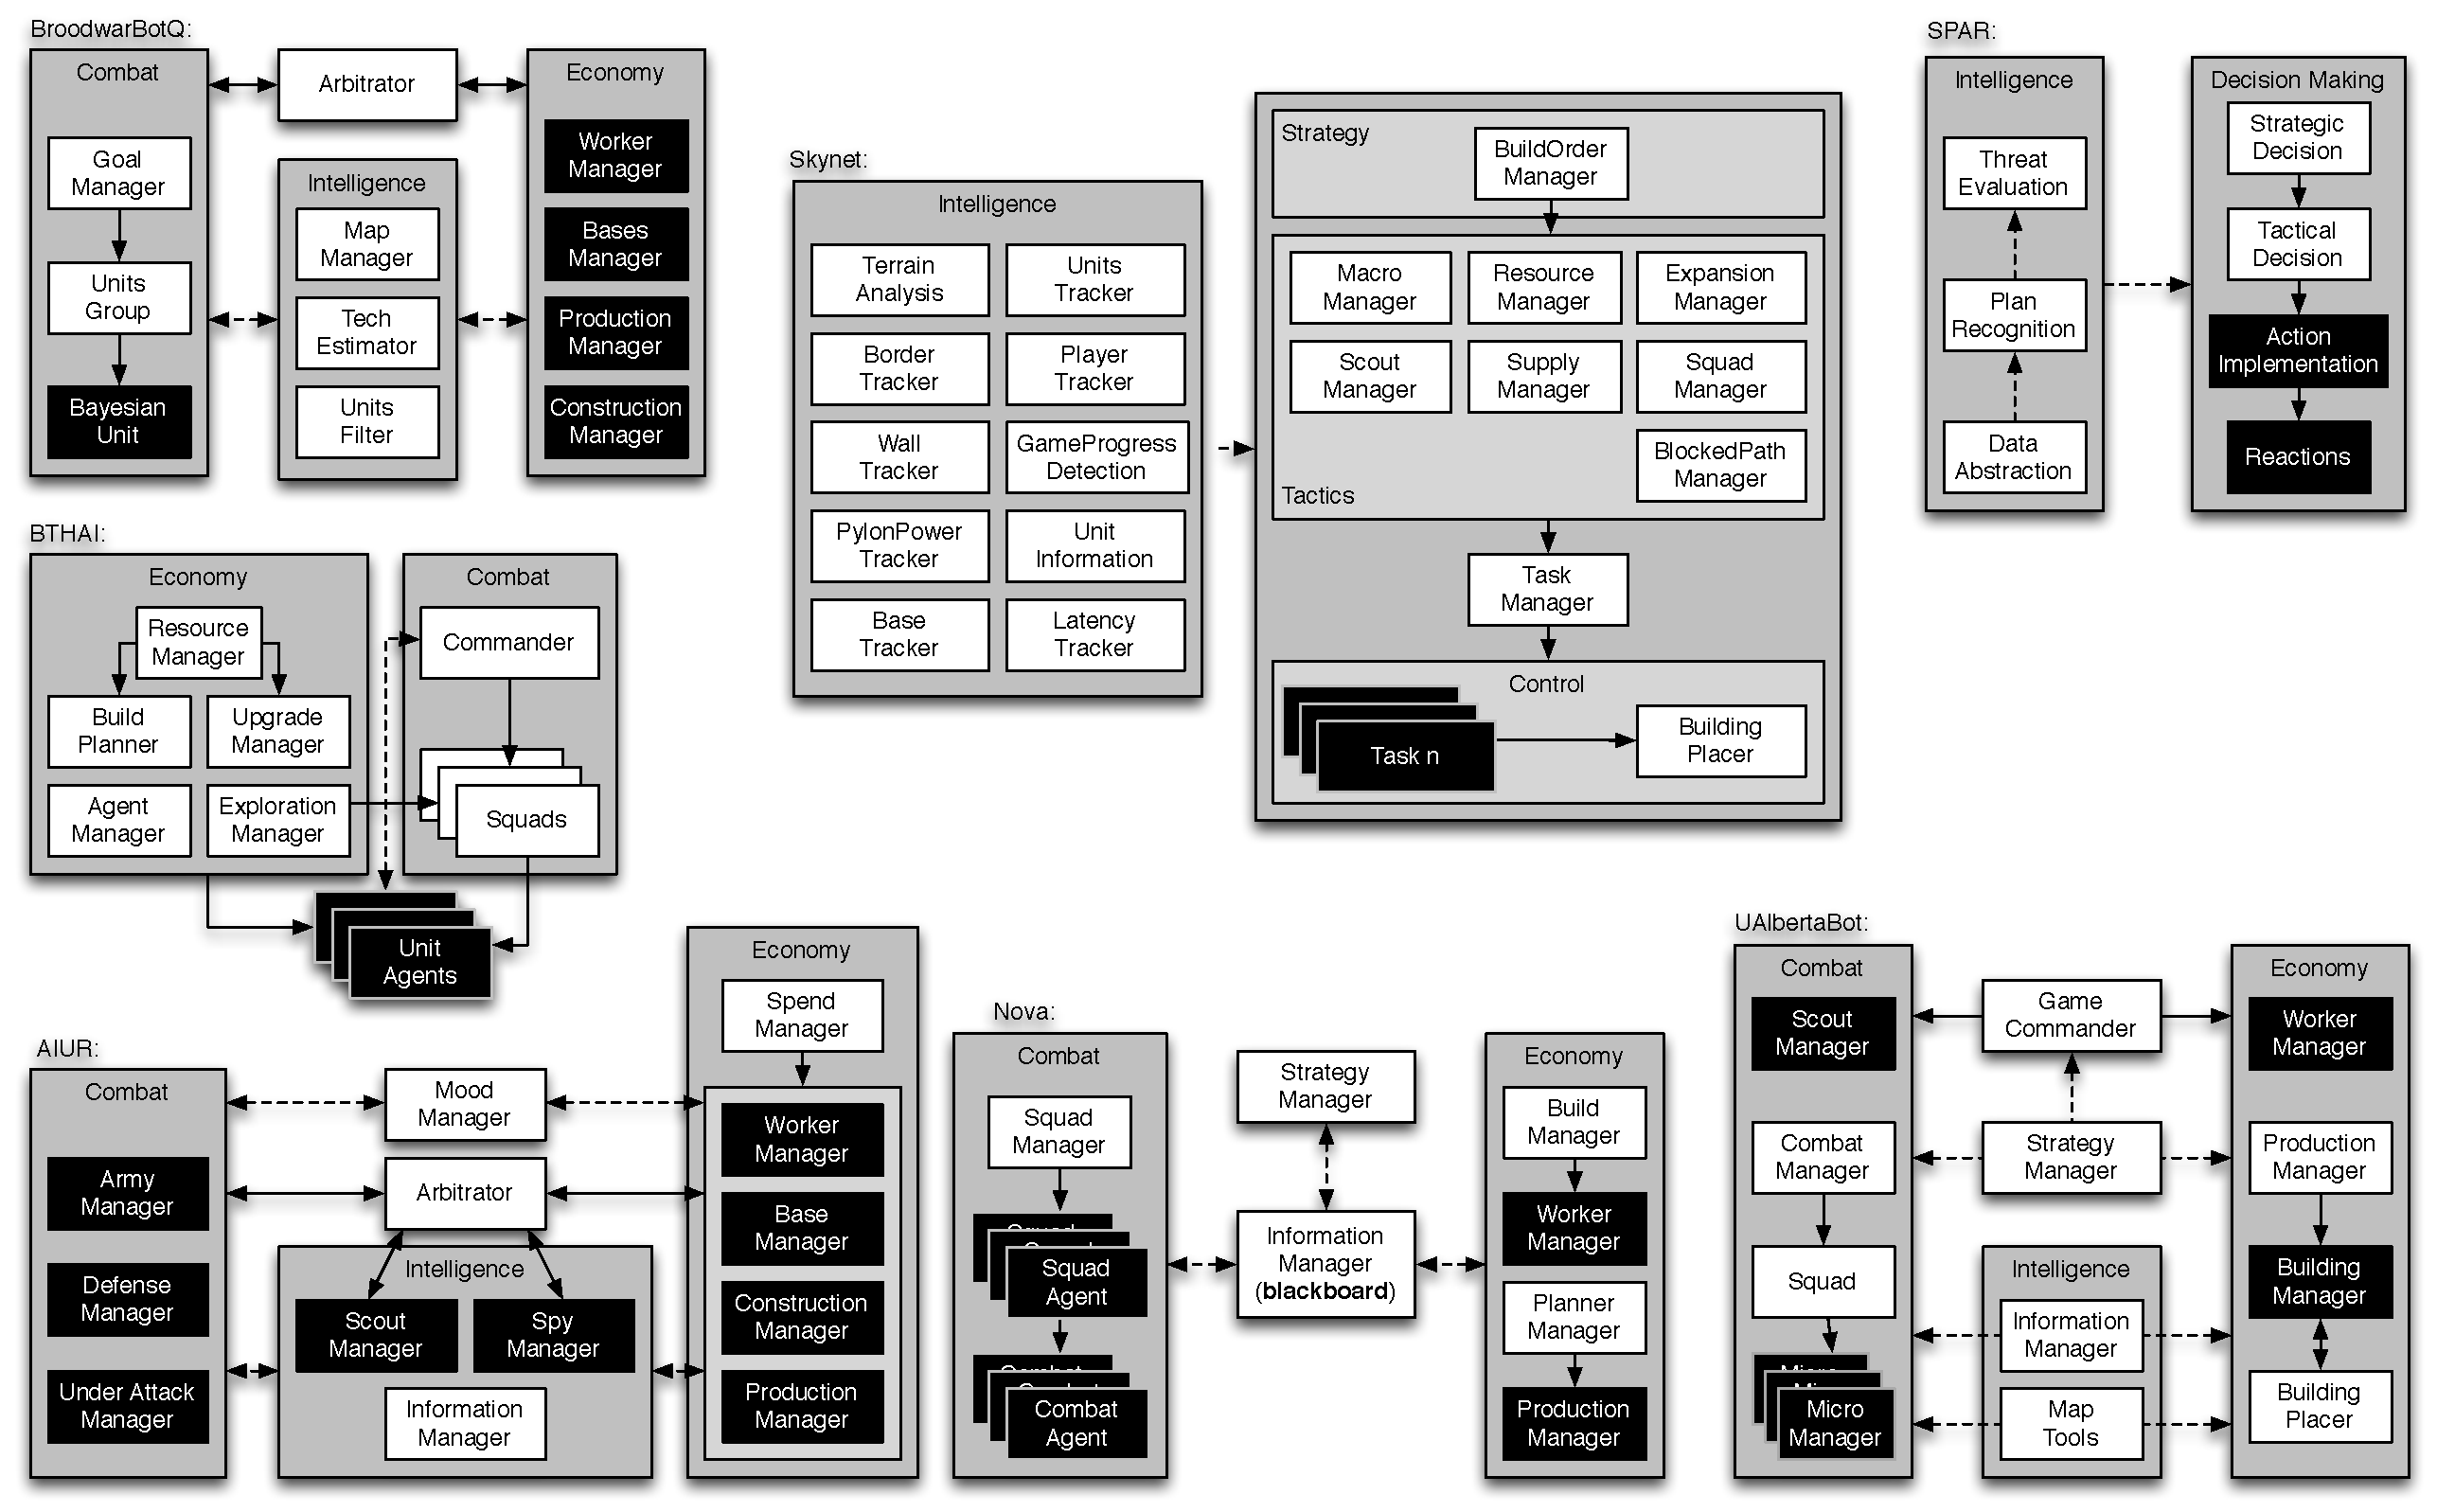
\includegraphics[width=\textwidth]{figures/figure-bot-architectures-wide.pdf}
    \caption{General architecture of 5 Starcraft AI bots.}
    \label{fig:bot-architecture}
\end{figure*}

Figure \ref{fig:bot-architecture} shows some representative examples of the integration architectures used by different bots in the AIIDE 2011 Starcraft AI competition \cite{???}. Each box represents an individual module with a clearly defined task (only modules with a black background can send actions directly to Starcraft). Dashed arrows represent data flow, and solid arrows represent control (when a module can command another module to perform some task). For example, we can see how SPAR is divided in two sets of modules: {\em situation analysis} and {\em decision making}, the first with three modules dedicated to analyze the current situation of the game, and the later with 4 modules dedicated to exploit that information to decide what to do. We can see how the decision making aspect of SPAR is organized hierarchically, with the higher-level module ({\em strategic decision}) issuing commands to the next module ({\em tactical decision}), which sends commands to the next module ({\em action implementation}), and so on. Only the lower-level modules can send actions directly to Starcraft. 

On the other hand, bots such as NOVA or BroodwarBotQ (BBQ) only use a hierarchical organization for {\em micro-management} (controlling the attack units), but use a decentralized organization for the rest of the bot. In Nova and BBQ, there is a collection of modules that control different aspects of the game (workers, production, construction, etc.). These modules can all send actions directly to Starcraft. In Nova those modules coordinate only through writing data in a shared blackboard, and in BBQ they coordinate only when they have to use a shared resource (unit) by means of an arbitrator.

By analyzing the structure of these bots, we can see that there are two main tools that can be used when designing an integration architecture:

\begin{itemize}
\item {\em Abstraction}: complex tasks can be formulated at different levels of abstraction. For example, playing an RTS game can be seen as issuing individual low-level actions to each of the units in the game, or at a higher level, it can be seen as deploying a specific strategy (e.g. a ``BBS strategy'', or a ``Reaver Drop'' strategy). Some bots, reason at multiple levels of abstraction at the same time, making the task of playing Starcraft simpler. Assuming that each module in the architecture of a bot has a goal and determines some actions to achieve that goal, the actions determined by higher-level modules are considered as the goals of the lower level modules. In this way, each module can focus on reasoning at only one level of abstraction, thus, making the problem easier.

\item {\em Divide-and-conquer}: playing a complex RTS, such as Starcraft, requires performing many conceptually different tasks, such as gathering resources, attacking, placing buildings, etc. Assuming each of these tasks can be performed relatively independently and without interference, we can have one module focusing on each of the tasks independently, thus making the problem easier. 
\end{itemize}

If we imagine the different tasks to perform in a complex RTS game in a two-dimensional plane, where the vertical axis represents abstraction, and the horizontal axis represents the different aspects of the game (micro-management, resource gathering, etc.), abstraction can be seen as dividing the space with horizontal lines, whereas divide-and-conquer divides the space using vertical lines.

Different bots, use different combinations of these two tools. Looking back at Figure \ref{fig:bot-architecture}, we can see the following use of abstraction and divide-in-conquer in the bots:

\begin{itemize}
\item BTHAI: uses a two-tier abstraction hierarchy, where a collection of high-level modules command a collection of lower-level agents in charge of each of the units. At the high-level, BTHAI uses divide-and-conquer, having multiple high-level modules issuing commands to the lower-level units.
\item BBQ: uses abstraction for micro-management, and divide-and-conquer for macro-management and intelligence gathering. To avoid conflicts between modules (since the individual tasks of each of the modules are not completely independent), BBQ uses an arbitrator.
\item Nova: is similar in design as BBQ, and uses abstraction for micro-management, and divide-and-conquer for macro-management. The differences are that Nova does not have an arbitrator to resolve conflicts, but has a higher-level module ({\em strategy manager}), which posts information to the blackboard that the rest of modules follow (thus, making use of abstraction).
\item SPAR: only uses abstraction. Its high-level module determines the strategy to use, and the tactical decision module divides it into a collection of {\em abstract actions}, that are executed by the lower-level modules.
\item Skynet: makes extensive use of both abstraction and divide-and-conquer. Considering the decision making component of Skynet, we can see a high level module that issues commands to a series of tactics modules. The collection of tactic modules queue {\em tasks} (that are analogous to the abstract actions used in SPAR). Each different task has a specific low level module that knows how to execute it. Thus, Skynet uses a 3 layered abstraction hierarchy, and uses divide-and-conquer in all levels except the highest.
\end{itemize}

Additionally, except for BTHAI, all other agents use divide-and-conquer at a higher-level bot design and divide all the modules into two or three categories: {\em information gathering} and {\em decision}, or {\em information gathering}, {\em micro-management} and {\em macro-management}.

Notice that most bots using divide-and-conquer (except for BBQ), assume that each of the modules can act independently and that their actions can be executed without interference. BBQ is the exception, including an arbitrator that makes sure that modules do not send contradictory orders to the same unit. However, very little bots handle the problem of how to coordinate resource usage amongst modules, for instance BTHAI uses a first-come-first-serve policy for spending resources, the first module that requests resources is the one that gets them. The exceptions are Nova and Skynet implement some rudimentary prioritization based on the high level strategy.

One interesting aspect of the five bots described above is that, while all of them are reactive at the lower level (unit control), most if not all of them, are scripted at the highest level of abstraction. BTHAI reads build and squad formations from a predefined script, Nova's {\em Strategy Manager} is a predefined finite-state machine, BBQ's construction manager reads the build order from a predefined script, and Skynet's {\em BuildOrder Manager} is basically a predefined script. Such scripts describe the strategy that the bots will use, however, such strategy is always fixed. One could see this pre-scripting as if each bot defined a ``high-level programming language'' to describe Starcraft strategies, and the bots themselves are just interpreters of such strategy. Compared to current approaches for Chess or Go, this scripting seems a bit rigid and inflexible, but responds to the much higher complexity of the Starcraft game.

In conclusion, we can see that there are two basic tools that can be used in an integration architecture: abstraction and divide-and-conquer, which are widely used by the existing Starcraft bots. However, several open questions remain:

{\color{blue}
\begin{itemize}
\item Strengths and weaknesses?
\item Resource coordination in a divide-and-conquer approaches?
\item High-level strategies that do not depend on scripting? (not here, this should be discussed in Section \ref{sec:planning})
\end{itemize}
}



% Can use something like this to put references on a page
% by themselves when using endfloat and the captionsoff option.
\ifCLASSOPTIONcaptionsoff
  \newpage
\fi

%\begin{thebibliography}{1}
%\end{thebibliography}
\bibliographystyle{IEEEtran}                                                    
\bibliography{survey}

%\begin{IEEEbiographynophoto}{FirstName LastName}
%Biography text here.
%\end{IEEEbiographynophoto}

\begin{IEEEbiography}[{
\includegraphics[width=2cm, keepaspectratio]{jim.jpg}}]{Jim Raynor}
Jim Raynor was a Confederate marshal on Mar Sara at the time of the first zerg incursions on that world. He is now with Raynor's Raiders Inc.
\end{IEEEbiography}

\end{document}


